\documentclass[11pt,a4paper,titlepage]{memoir} %% memoire class

\usepackage[OT1]{fontenc}

\usepackage[american]{babel} %% language support, english also available

\usepackage[utf8]{inputenc}

\usepackage{amsmath,amssymb,amsfonts,mathrsfs} %% math typesetting

\usepackage{graphicx} %% latex graphics handling

\usepackage{pdfpages} %% allows to add .pdf files


%\usepackage{multirow} %% [OPT] Multi-rowed cells in tabulars

\usepackage{varioref} %%nice combines references
\usepackage{datetime} %% [REC] Format dates and time depending on locale 
\usepackage{cancel}   %% [OPT] Provides a \cancel{} command to stroke through mathematics.
\usepackage{mathtools} %% additional typesetting in math
\usepackage[h]{esvect} %% alternate vector arrows
\usepackage{array} %% [NEED] Some extensions to tabulars and array environments. 

\usepackage{listings} %% fancy package for source code listings
\lstset{language=TeX,basicstyle={\normalfont\ttfamily}}

\usepackage[activate]{pdfcprot} %% fancy character protrusion
\usepackage{booktabs} %% nicer tables




%% Memoir layout setup

%% NOTE: You are strongly advised not to change any of them unless you
%% know what you are doing.  These settings strongly interact in the
%% final look of the document.

% Dependencies
\usepackage{ETHlogo}

% Turn extra space before chapter headings off.
\setlength{\beforechapskip}{0pt}

\nonzeroparskip
\parindent=0pt
\defaultlists

% Chapter style redefinition
\makeatletter

\if@twoside
  \pagestyle{Ruled}
  \copypagestyle{chapter}{Ruled}
\else
  \pagestyle{ruled}
  \copypagestyle{chapter}{ruled}
\fi
\makeoddhead{chapter}{}{}{}
\makeevenhead{chapter}{}{}{}
\makeheadrule{chapter}{\textwidth}{0pt}
\copypagestyle{abstract}{empty}

\makechapterstyle{bianchimod}{%
  \chapterstyle{default}
  \renewcommand*{\chapnamefont}{\normalfont\Large\sffamily}
  \renewcommand*{\chapnumfont}{\normalfont\Large\sffamily}
  \renewcommand*{\printchaptername}{%
    \chapnamefont\centering\@chapapp}
  \renewcommand*{\printchapternum}{\chapnumfont {\thechapter}}
  \renewcommand*{\chaptitlefont}{\normalfont\huge\sffamily}
  \renewcommand*{\printchaptertitle}[1]{%
    \hrule\vskip\onelineskip \centering \chaptitlefont\textbf{\vphantom{gyM}##1}\par}
  \renewcommand*{\afterchaptertitle}{\vskip\onelineskip \hrule\vskip
    \afterchapskip}
  \renewcommand*{\printchapternonum}{%
    \vphantom{\chapnumfont {9}}\afterchapternum}}

% Use the newly defined style
\chapterstyle{bianchimod}

\setsecheadstyle{\Large\bfseries\sffamily}
\setsubsecheadstyle{\large\bfseries\sffamily}
\setsubsubsecheadstyle{\bfseries\sffamily}
\setparaheadstyle{\normalsize\bfseries\sffamily}
\setsubparaheadstyle{\normalsize\itshape\sffamily}
\setsubparaindent{0pt}

% Set captions to a more separated style for clearness
\captionnamefont{\sffamily\bfseries\footnotesize}
\captiontitlefont{\sffamily\footnotesize}
\setlength{\intextsep}{16pt}
\setlength{\belowcaptionskip}{1pt}

% Set section and TOC numbering depth to subsection
\setsecnumdepth{subsection}
\settocdepth{subsection}

%% Titlepage adjustments
\pretitle{\vspace{0pt plus 0.7fill}\begin{center}\HUGE\sffamily\bfseries}
\posttitle{\end{center}\par}
\preauthor{\par\begin{center}\let\and\\\Large\sffamily}
\postauthor{\end{center}}
\predate{\par\begin{center}\Large\sffamily}
\postdate{\end{center}}

\def\@advisors{}
\newcommand{\advisors}[1]{\def\@advisors{#1}}
\def\@department{}
\newcommand{\department}[1]{\def\@department{#1}}
\def\@university{}
\newcommand{\university}[1]{\def\@university{#1}}
\def\@thesistype{}
\newcommand{\thesistype}[1]{\def\@thesistype{#1}}

\renewcommand{\maketitlehooka}{\noindent\ETHlogo[2in]}

\renewcommand{\maketitlehookb}{\vspace{1in}%
  \par\begin{center}\Large\sffamily\@thesistype\end{center}}

\renewcommand{\maketitlehookd}{%
  \vfill\par
  \begin{flushright}
    \sffamily
    \@advisors\par
    \@department \par
    \@university
  \end{flushright}
}

\checkandfixthelayout

\setlength{\droptitle}{-48pt}

\makeatother
 %% layout configuration

% custom made commands


\newcommand{\met}{\mathbb{MET}}

 %% commands like \met and \ht and whatnot

\usepackage[linkcolor=black,colorlinks=true,citecolor=black,filecolor=black]{hyperref} %% document internal hyperlinks wherever possible


%% Document information
%% ====================

\title{Same-sign dileptons as a search tool at CMS}
\author{Marc D\"unser}
\thesistype{Doctoral Thesis}
\advisors{Advisors: Prof.\ Dr.\ Rainer Wallny}
\department{Institute for Particle Physics, D-PHYS}
\university{ETH Z\"urich}
\date{\today}

\begin{document}

\frontmatter

%% titlepage is defined in layoutsetup.tex. look in there for info
\begin{titlingpage}
  \calccentering{\unitlength}
  \begin{adjustwidth*}{\unitlength-24pt}{-\unitlength-24pt}
    \maketitle
  \end{adjustwidth*}
\end{titlingpage}

%% declaration of originality must be included somewhere
%% 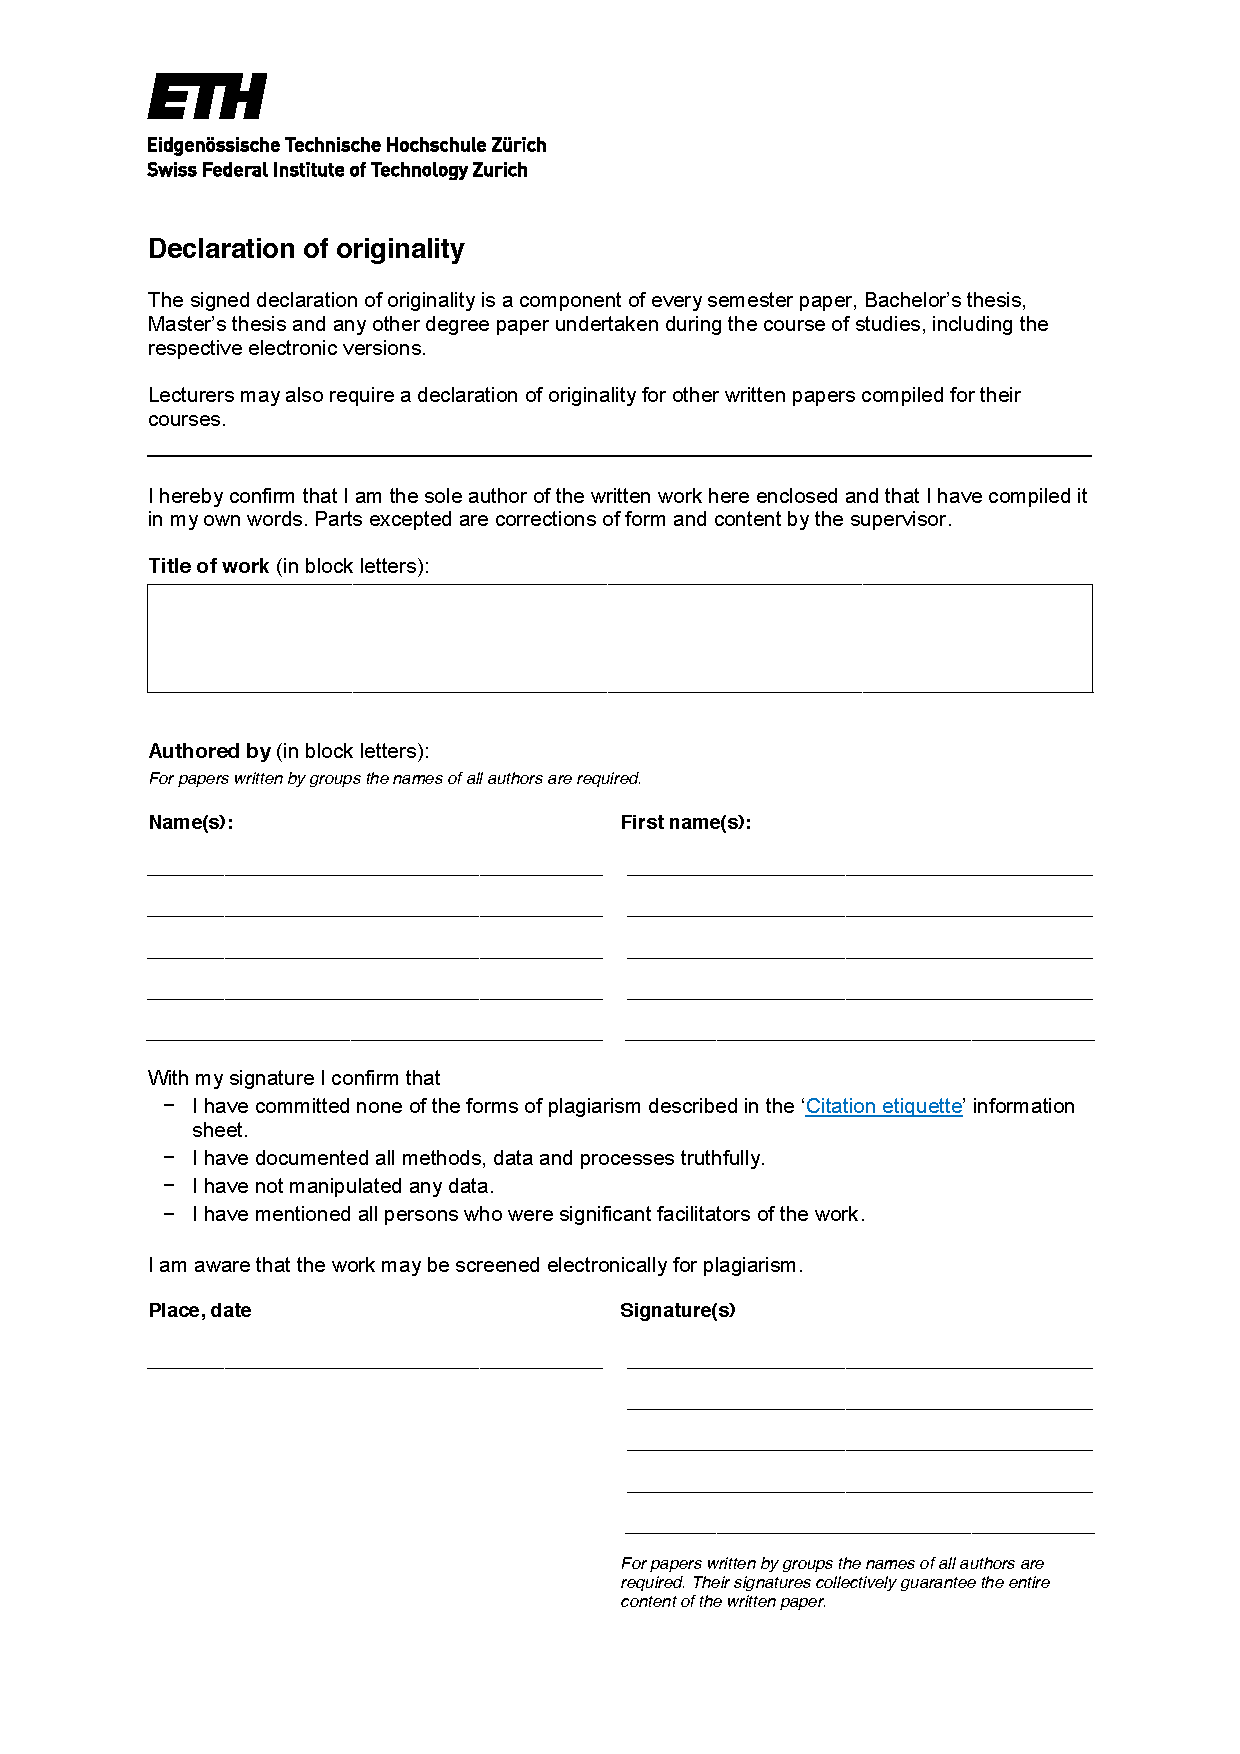
\includepdf[pages={-}]{declaration-originality.pdf}

\begin{abstract}
  This example thesis briefly shows the main features of our thesis
  style, and how to use it for your purposes.
\end{abstract}
 %% include the abstract

%% TOC
\cleartorecto
\tableofcontents
\mainmatter

%% the capters
% Some commands used in this file
\newcommand{\package}{\emph}

\chapter{Introduction}

The construction of the LHC and its experiments over the few last decades has been only
the last step in a long and successful history of particle accelerators that started roughly 100 years
ago with the construction of the first 



\section{Features}
\label{sec:features}





\chapter{Theory}
\label{ch:theory}
In order to interpret any experimental result, it is of paramount importance to understand
the underlying model governing the physical processes in question. Modern physics knows a
large number of rather successful theories all dedicated to describing different mass and 
energy scales. An example is the theory of classical mechanics, which manages to describe the 
physics of `daily life' very well. However, it breaks down when velocities approach
the speed of light and has to be incorporated into a broader theory, namely that of relativity.

This specific example already suggests that different physical theories are valid only in a 
certain energy range and describe only a certain `type'\footnote{In this particular example
electromagnetic interactions are -- for instance -- not described at all.} of physical process. 
This fact is also true for the case of particle physics. The relevant theory is called the 
\textit{`Standard Model'} and will be described hereafter. Further into the chapter,
a short description of the pitfalls of the standard model will be given with some explanation
on possible solutions.

\section{The Standard Model}
\label{sec:standardmodel}
The Standard Model (SM) of particle physics provides the theoretical framework that
describes all fundamental particles and the forces that act between them, with the one
exception of gravity. Despite a few drawbacks that will be described later (see Section~\ref{sub:sm_shorts})
it has been an overwhelmingly successful theory, capable of describing experimental data
with a precision that is simply outstanding.

\subsection{Particle content in the Standard Model}
\label{sub:sm_particles}
\subsection{Shortcomings of the Standard Model}
\label{sub:sm_shorts}
\section{Supersymmetry}
\label{sec:susy}
\subsection{Particle content}
\label{sub:susy_particles}
\subsection{Observables for searches for Supersymmetry}
\label{sub:susy_observables}
\section{Remaining open questions in particle physics}
\label{sec:theory_remains}

\chapter{The Experiment}
\label{ch:cms}


\num{0.3e45}

\chapter{Same-sign dilepton analyses}
\label{ch:analysis}

\section{Search for Supersymmetry in events with hadronic activity}
\label{sec:ra5}
\section{Search for electroweak production of Supersymmetry}
\label{sec:ewino}

\section{Fake leptons}
\label{sec:fakes}

\chapter{Outlook}
\label{ch:outlook}

\chapter{Conclusions}
\label{ch:conclusions}

\input{chapters/acknowledgments}

\appendix

\chapter{Dummy Appendix}

You can defer lengthy calculations that would otherwise only interrupt
the flow of your thesis to an appendix.


\backmatter

\bibliographystyle{plain}
\bibliography{refs}

\end{document}
